% Created 2021-03-30 Tue 18:45
% Intended LaTeX compiler: pdflatex
\documentclass[11pt]{article}
\usepackage[utf8]{inputenc}
\usepackage[T1]{fontenc}
\usepackage{graphicx}
\usepackage{grffile}
\usepackage{longtable}
\usepackage{wrapfig}
\usepackage{rotating}
\usepackage[normalem]{ulem}
\usepackage{amsmath}
\usepackage{textcomp}
\usepackage{amssymb}
\usepackage{capt-of}
\usepackage{hyperref}
\usepackage{minted}
\author{Tony Valentine}
\date{\today}
\title{Tealang Interpreter}
\hypersetup{
 pdfauthor={Tony Valentine},
 pdftitle={Tealang Interpreter},
 pdfkeywords={},
 pdfsubject={},
 pdfcreator={Emacs 26.3 (Org mode 9.5)}, 
 pdflang={English}}
\begin{document}

\maketitle
\tableofcontents

\newpage
\section{Language Definition}
\label{sec:orgcd7c3fd}

The Tealang language is defined using the following EBNF. The '[]' wrapper is equivalent to '?' in regex, and the '\{\}' wrapper is equivalent to '*' in regex.

\begin{verbatim}
<Letter>            ::= [A-Za-z]
<Digit>             ::= [0-9]
<Printable>         ::= [\x20-\x7E]
<Type>              ::= 'float' | 'int' | 'bool' | 'string'
<BooleanLiteral>    ::= 'true' | 'false'
<IntegerLiteral>    ::= <Digit> { <Digit> }
<FloatLiteral>      ::= <Digit> { <Digit> } '.' <Digit> { <Digit> }
<StringLiteral>     ::= '"' {<Printable> } '"'
<Literal>           ::= <BooleanLiteral>
                        |<IntegerLiteral>
                        |<FloatLiteral>
                        |<StringLiteral>
<Identifier >       ::= ('_'| <Letter>) {'_'| <Letter> | <Digit> }
<MultiplicativeOp>  ::= '*' | '/' | 'and'
<AdditiveOp>        ::= '+' | '-' | 'or'
<RelationalOp>      ::= '<' | '>' | '==' | '!=' | '<=' | '>='
<ActualParams>      ::= <Expression> { ',' <Expression> }
<FunctionCall >     ::= <Identifier > '(' [ <ActualParams> ] ')'
<SubExpression>     ::= '(' <Expression> ')'
<Unary>             ::= ( '-' | 'not' ) <Expression>
<Factor >           ::= <Literal >
                        |<Identifier >
                        |<FunctionCall >
                        |<SubExpr>
                        |<Unary>
<Term>              ::= <Factor > { <MultiplicativeOp> <Factor > }
<SimpleExpression>  ::= <Term> { <AdditiveOp> <Term> }
<Expression>        ::= <SimpleExpression> { <RelationalOp> <SimpleExpression> }
<Assignment>        ::= <Identifier > '=' <Expression>
<VariableDecl >     ::= 'let' <Identifier > ':' <Type> '=' <Expression>
<PrintStatement>    ::= 'print' <Expression>
<RtrnStatement>     ::= 'return' <Expression>
<IfStatement>       ::= 'if' '(' <Expression> ')' <Block > [ 'else' <Block > ]
<ForStatement>      ::= 'for' '(' [ <VariableDecl > ] ';' <Expression> ';'
                        [<Assignment> ] ')' <Block >
<WhileStatement>    ::= 'while' '(' <Expression> ')' <Block >
<FormalParam>       ::= <Identifier > ':' <Type>
<FormalParams>      ::= <FormalParam> { ',' <FormalParam> }
<FunctionDecl >     ::= <type> <Identifier > '(' [ <FormalParams> ] ')' <Block >
<Statement>         ::= <VariableDecl > ';'
                        |<Assignment> ';'
                        |<PrintStatement> ';'
                        |<IfStatement>
                        |<ForStatement>
                        |<WhileStatement>
                        |<RtrnStatement> ';'
                        |<FunctionDecl >
                        |<Block >
<Block >            ::= '{' { <Statement> } '}'
<Program>           ::= { <Statement> }

\end{verbatim}


\newpage
\section{Lexer}
\label{sec:orgb899628}

\subsection{Lexer Components}
\label{sec:orgd672535}

\subsubsection{Identifiers and Keywords}
\label{sec:orgf6936df}

Keywords are reserved identifiers required for operation of the language. Since the set of all keywords is a subset of all identifiers we can focus on detecting correct identifiers first and then check for keywords. The regex for an identifier is \texttt{(\_|[A-z])(\_|[A-z]|[0-9])+}. To determine the exact token a map can be used to locate the correct token in logarithmic time.

\begin{figure}[htbp]
\centering
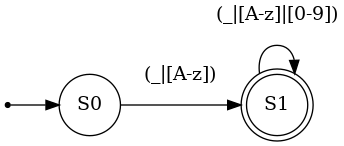
\includegraphics[width=200px]{automaton/identifier.png}
\caption{\label{fig:iden-dfa}Identifier DFA}
\end{figure}


\subsubsection{Integers and Floats}
\label{sec:org2e2f07d}

Taking a look at the BNF it can be seen that a the definition for \texttt{float} is a concatenation of \texttt{int} with \texttt{.} and another \texttt{int}. As such a dfa can be defined to accept both of these strings, and they can be interpreted according the final state of the automaton. In the automaton below if the system stops in state \texttt{Int} we know it must be an integer, whereas stopping in state \texttt{Float} assures that the number is a float.

\begin{figure}[htbp]
\centering
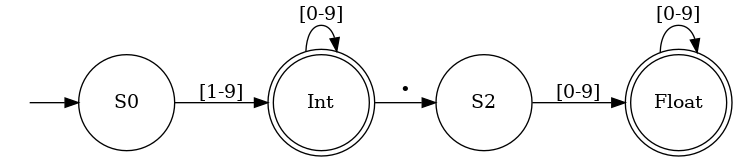
\includegraphics[width=250px]{automaton/nums.png}
\caption{\label{fig:nums-dfa}Integer and Float DFA}
\end{figure}


\subsubsection{Relational Operators and Equality}
\label{sec:org2a613d8}

The relational operators require a slightly more complex DFA than previous examples. This is specifically due to the \texttt{!=} and singular \texttt{=} operator. However these can easily be resolved with 2 extra cases in the DFA.

\begin{figure}[htbp]
\centering
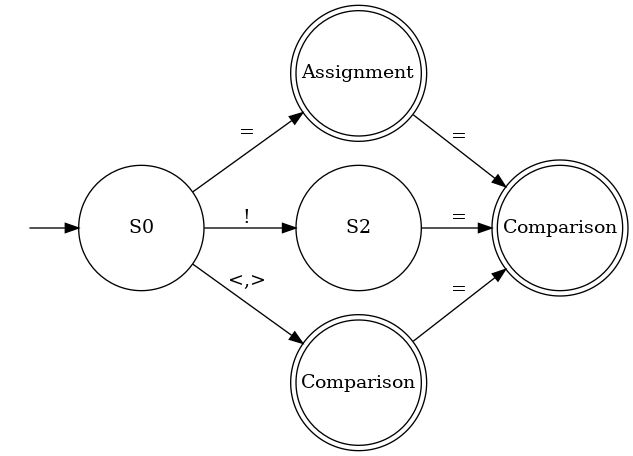
\includegraphics[width=150px]{automaton/eq_comp.png}
\caption{\label{fig:eq-comp-dfa}Comparison and Assignment DFA}
\end{figure}
\end{document}
